\section{Ground Heat Transfer Calculations using Site:GroundDomain:Basement}\label{ground-heat-transfer-calculations-using-sitegrounddomainbasement}

Basement heat transfer calculations are performed by the same model used by Site:GroundDomain:Slab to simulate zone-ground coupled surfaces. To simulate basements, the previous model is extended to situations where surfaces are below ground.

\subsubsection{Approach}\label{approach-000}

This model is generalized to be able to handle several basement surface and insulation configurations. An implicit finite difference formulation is used to solve for the ground temperatures. As a result the simulation is stable for all timesteps and grid sizes, but an iteration loop must be employed to converge the temperatures in the domain for each domain timestep.

Multiple basement zones can be coupled to each basement domain object. The model determines which floor surfaces are coupled to the basement domain and creates a floor surface of equivalent surface area within the basement domain as a representation of the horizontal surfaces coupled to the domain. The user defined aspect ratio, which is the ratio of basement width to length, along with the total surface area of all surfaces connected to this basement floor will define the size and shape of the basement ground domain.

Vertical basement depth below the ground surface of the domain is user specified. For situations when the ground surface is lower than the first above ground level a separate surface should be employed to bridge the space between the ground domain, and the first above-ground level.

Basement wall and floor surfaces are created normally using the BuildingSurface:Detailed objects, with the outside boundary condition being the OtherSideConditionsModel used for the walls and floor of the basement domain. The interface between the basement walls and floors occurs at the outside surface of the walls and floor. Outside underground insulation is simulated by the ground domain, and therefore should not be included in the basement wall and floor construction objects.

\subsubsection{Boundary Conditions}\label{boundary-conditions}

At the zone interface surfaces, the average surface conduction heat flux from all surfaces connected to the ground domain is imposed as a boundary condition at the Surface/Domain interface cells. Far-field temperatures are applied as boundary temperature at the domain sides and lower surface. The ground temperature profile at the domain sides and lower surface are taken from Kusuda \& Achenbach 1965. The correlation requires annual ground surface temperature data. Ground surface temperature data can be determined by using the CalcSoilSurfTemp preprocessor; or, if the user has average monthly ground surface temperature data available, they can use the Site:GroundTemperature:Shallow object to provide the model monthly ground surface temperatures. From that, the model can then determine the ground temperature model parameters for the Kusuda \& Achenbach (1965) ground temperature model.

Ground surface cells are treated as a heat balance, where long and short wave radiation, conduction, and convection are considered. Evapotranspiration is also considered. The evapotranspiration rate is calculated as a moisture loss by using the Allen et al. (2005) model, and translated into a heat loss by multiplication with the density and latent heat of evaporation of water. The evapotranspiration rate is dependent on the type of vegetation at the surface; the user can vary the surface vegetation from anywhere between a concrete surface and a fairly tall grass (about 7''). The model can be sensitive to variations in this parameter, especially in hot dry climates.

Once the basement model has run, the updated cells with zone surface boundary conditions will update the OtherSideConditionsModel temperatures which are then used at the next timestep in the surface heat balance calculations.

\subsubsection{Simulation Methodology}\label{simulation-methodology}

The ground domain is updated at each zone timestep, or hourly as specified by the user. For situations when the ground domain is updated at each timestep, the domain is simulated by applying the surface heat flux boundary conditions from the previous timestep and calculating a new OthersideConditionsModel temperature. At this point, the surface heat balance algorithms can then take the new outside surface temperatures to update their surface heat fluxes. For situations when the user has elected to have the domain update on an hourly basis, the surface heat flux for each coupled surface is aggregated and passed to the domain as an average surface heat flux from the previous hour, which will then update the outside surface temperatures for the surface heat balance's next iteration.

The basement floor and walls are simulated by standard surface heat balance models within EnergyPlus (CTF, finite difference). The horizontal and vertical insulation are simulated by the ground domain finite difference solver. This is shown in Figure~
\ref{BasementGHTFigure1} below where the dotted red line defines the OtherSideConditionsModel interface separating the two solution domains. This methodology applies to the basement floor and walls.

\begin{figure}[htbp]
\centering
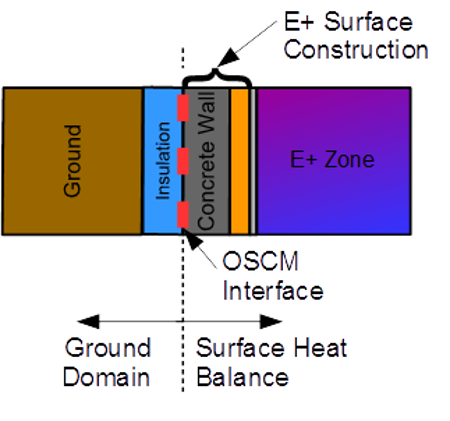
\includegraphics{media/image8000.png}
\caption{Example surface construction.}
\label{BasementGHTFigure1}
\end{figure}

References

Kusuda, T. \& Achenbach, P. 1965. `Earth Temperature and Thermal Diffusivity at Selected Stations in the United States', ASHRAE Transactions 71(1): 61--75.

Allen, R.G., Walter, I.A., Elliott, R.L., Howell, T.A., Itenfisu, D., Jensen, M.E., Snyder, R.L. 2005. The ASCE standardized reference evapotranspiration equation. Reston, VA: American Society of Civil Engineers.
